\documentclass[user_manual.tex]{subfiles}
\begin{document}


 \chapter{Aspectos generales}
En este capitulo se abordaran los aspectos más comunes del robot Justina sobre el hardware que integra a Justina y marcaremos aspectos importantes para su correcto funcionamiento y un desempeño óptimo. Se explorara la configuración mecánica de Justina y se especificara el funcionamiento de cada una.\\
\\
El cuerpo de Justina esta conformado por una cabeza mecatronica, brazos mecatronicos, un torso que se utiliza para variar la altura del robot Justina y una base que se encarga del desplazamiento de Justina; además de contener la etapa de potencia y la mayoria del control sobre el roboto Justina.


\begin{center}
\includegraphics[width=0.4\textwidth]{Figures/Hardware/Diagramas/Cuerpo.png}
\captionof{figure}{(a):Cabeza mecatronica-(b):Brazo mecatronico-(c):Torso-(d):Base holonomica}
\label{fig:Hardware:Diagramas:Justina:Completa}
\end{center}
\section{Cabeza mecatronica}
 La cabeza mecatronica está formada por un sensor kinect el cual tiene integrado varios componentes para ayudar a
 llevar a cabo tareas. Cuenta con una cámara la cual será utilizada para la visión y la detección de objetos apoyado por la cámara de color, estos son utilizados para reconocimiento de patrones y compararlos en la 
 base de datos para reconocer el objeto.\\
 \\
 La cabeza mecatronica cuenta con 2 grados de libertad, uno hace un movimiento de inclinación conocido cómo "titl" y otro para un movimiento rotacional conocido cómo "pan".

\begin{center}
\includegraphics[width=0.6\textwidth]{Figures/Hardware/Partes/Kinect_sensors.png}
\captionof{figure}{Componentes internos del sensor kinect}
\label{fig:Hardware:Diagramas:Justina:Vision:Kinect}
\end{center}

Para la adquisición de audio cuenta con un micrófono RODE. Para el movimiento cuenta con dos servomotores
para darle dos grados de libertad, cuenta con un MX-106 y un MX-64. Para controlar los servomotores se hace uso de un
USB2Dynamixel el cual tiene una conexion R232.

\begin{center}
\includegraphics[width=0.7\textwidth]{Figures/Hardware/Diagramas/Cabeza.png}
\captionof{figure}{Cabeza mecatronica de Justina}
\label{fig:Hardware:Diagramas:Justina:Completa}
\end{center}

\newpage
\section{Brazos mecatronicos}
Los brazos mecatronicos cuentan con 10 servomotores para darle 7 grados de libertad simulando un brazo humano, además de contar con un griper capaz de agarrar objetos. Está articulado para que cumpla casi los mismos movimientos de un brazo humano.

\begin{center}
\includegraphics[width=0.9\textwidth]{Figures/Hardware/Diagramas/Brazo.png}
\captionof{figure}{Brazo mecatronico}
\label{fig:Hardware:Diagramas:Justina:Brazo}
\end{center}

\subsection{Cinemática directa y cinemática inversa de los brazos}
%Principio de la tabla del MX-106
\begin{table}[H]
\begin{center}
\begin{tabular}{l|l l l l}%Define el número de columnas

Art & a & d & $\alpha$ & $\theta$\\ \hline 
1 & 0.0603 & 0     & $\pi \over 2$ & 0\\
2 & 0      & 0     & $\pi \over 2$ & $\pi \over 2$\\
3 & 0      & 0.285 & -$\pi \over 2$& -$\pi \over 2$\\
4 & 0      & 0     & $\pi \over 2$ & 0\\
5 & 0      & 0     & -$\pi \over 2$& 0\\
6 & 0      & 0     & $\pi \over 2$ & 0\\
7 & 0      & 0.12  &        0      & 0\\
\end{tabular}
\caption{Datos}
\end{center}
\end{table}
%Fin de la tabla

\textbf{Cinemática Inversa}\\
\\
$r=\sqrt{x^2+y^2+(z-D_1)^2}$\\
$\alpha=Atan2((z-D_1),\sqrt{x^2+y^2})$\\
$\gamma=arccos\frac{-D_2^2-D_3^2+r^2}{-2*D_2*D_3}$\\
$\beta=\frac{arcsin(D_3)*sin(\gamma)}{r}$
$tunningRadiusElbow=D_2*sin\beta$\\
$Pelbow[0,0]=Pw[0,0]=0$\\
$Pelbow[1,0]=Pw[1,0]=-tunningRadiusElbow*\cos elbowAngle=D_2*\sin\beta*\cos elbowAngle$\\
$Pelbow[2,0]=Pw[2,0]=-tunningRadiusElbow*\sin elbowAngle=D_2 *\sin\beta*\sin elbowAngle$\\
$Pelbow[3,0]=Pw[3,0]=1$\\
$WristPosition[1,0]=WP[1,0]=y;$\\
$WristPosition[2,0]=WP[2,0]=z;$\\
$WristPosition[3,0]=WP[3,0]=1;$\\
\\
$result[0]=Atan2(Pw[1,0]+DH_a[0]*\sin result[0],Pw[0,0]+DH_a[0]*\cos result[0])$\\
$result[1]=Atan2(Pw[2,0]-D_1,\sqrt{Pelbow[0,0]*Pelbow[0,0]+Pw[1,0]*Pw[1,0]})$\\
$result[2]=Atan2(WP[1,0],WP[0,0])$\\
$result[3]=\frac{\pi}{2}-Atan2(WP[2,0],\sqrt{WP[0,0]*WP[0,0]+WP[1,0]*WP[1,0]})$\\
\\
\textbf{Condiciones}\\
\\
if $R47[0,0]==0\\
result[4]=0\\
result[5]=0\\
result[6]=Atan2(R47[1,1],R47[1,2])$\\
\\
else
$result[5]=Atan2(\sqrt{1-(R47[2,0])^2},R47[2,0])\\
result[4]=Atan2(R47[1,0],R47[0,0])\\
result[6]=Atan2(R47[2,2],-R47[2,1])$\\
\\
if $result[4]>2.4\\
result[4]+=\pi\\
resulr[5]*=-1$\\
if $result[6]>0\\
result[6]-=\pi$\\
else $result[6]+=\pi$\\
\\
if $result[4]<-2.4\\
result[4]+=\pi\\
result[5]*=-1$\\
if $result[6]>0\\
result[6]-=\pi$\\
else $result[6]+=\pi$\\
\\
La cinemática directa y la inversa son las mismas para cada brazo, el úico cambio es el sentido de giro de algunas articulaciones. La configuración de los brazos es la misma, un brazo está desplazado respecto del otro.

\begin{center}
\includegraphics[width=0.3\textwidth]{Figures/Hardware/Cinematica/Cine_1.png}
\captionof{figure}{Eje X,Y,Z}
\end{center}

\newpage

\begin{center}
\includegraphics[width=0.3\textwidth]{Figures/Hardware/Cinematica/Cine_2.png}
\captionof{figure}{Brazo izquierdo}
\end{center}

\begin{center}
\includegraphics[width=0.3\textwidth]{Figures/Hardware/Cinematica/Cine_3.png}
\captionof{figure}{Articulaciones 1,2,3}
\end{center}

\begin{center}
\includegraphics[width=0.25\textwidth]{Figures/Hardware/Cinematica/Cine_4.png}
\captionof{figure}{Articulaciones 4,5}
\end{center}

\begin{center}
\includegraphics[width=0.25\textwidth]{Figures/Hardware/Cinematica/Cine_5.png}
\captionof{figure}{Articulaciones 6,7}
\end{center}

\begin{center}
\includegraphics[width=0.6\textwidth]{Figures/Hardware/Cinematica/Cine_6.png}
\captionof{figure}{Sentido de giro brazo izquierdo-derecho}
\end{center}

\begin{center}
\includegraphics[width=0.4\textwidth]{Figures/Hardware/Cinematica/Cine_7.png}
\captionof{figure}{Giro de articulaciones 1,2,3}
\end{center}

\begin{center}
\includegraphics[width=0.35\textwidth]{Figures/Hardware/Cinematica/Cine_8.png}
\captionof{figure}{Giro de articulaciones 4,5,6}
\end{center}

\begin{center}
\includegraphics[width=0.4\textwidth]{Figures/Hardware/Cinematica/Cine_9.png}
\captionof{figure}{Giro de articulacion 7}
\end{center}

\section{Torso y base holónomica}
El torso de justina aparte de ser el eje central y soporte de los brazos y la cabeza tiene una guía para llevar todo el cableado de la cabeza y los brazos a la base. El torso sirve principlmente para ayudar al robot Justina a agarrar los objetos con el griper más fácilmente al cambiar la altura del robot. \\
\\
La base holonómica es donde se encuentra toda la etapa de potencia y ejecuta el desplazamieto del robot Justina. Para la etapa de potencia cuenta con unas clemas, las cuales distribuyen el voltaje entre todos los dispositivos que integran a Justina. Las clemas más grandes son utilizadas para conectar todas las tierras y las más pequeñas son utilizadas para distribuir el voltaje. La alimentación de los servomotores es controlada utilizando dos tipos
de robloclaw.\\
\\ Para el desplazamiento de Justina se utilizaron cuatro motores, los cuales tienen ensambladas llantas cada uno las cuales le permiten un desplazamiento en cualquier dirección.

\begin{center}
\includegraphics[width=0.9\textwidth]{Figures/Hardware/Diagramas/Base.png}
\captionof{figure}{Interior de la base de Justina}
\label{fig:Hardware:Diagramas:Justina:Base}
\end{center}

\section{Diagramas esquemáticos}
Se muestran los diagramas esquemáticos de las conexiones del hardware de Justina; tanto los diagramas esquematicos de energía como los diagramas esquematicos de las roboclaws utilizadas.


\subsection{Diagrama esquemático conexiones en las clemas}

%Figura
\begin{center}
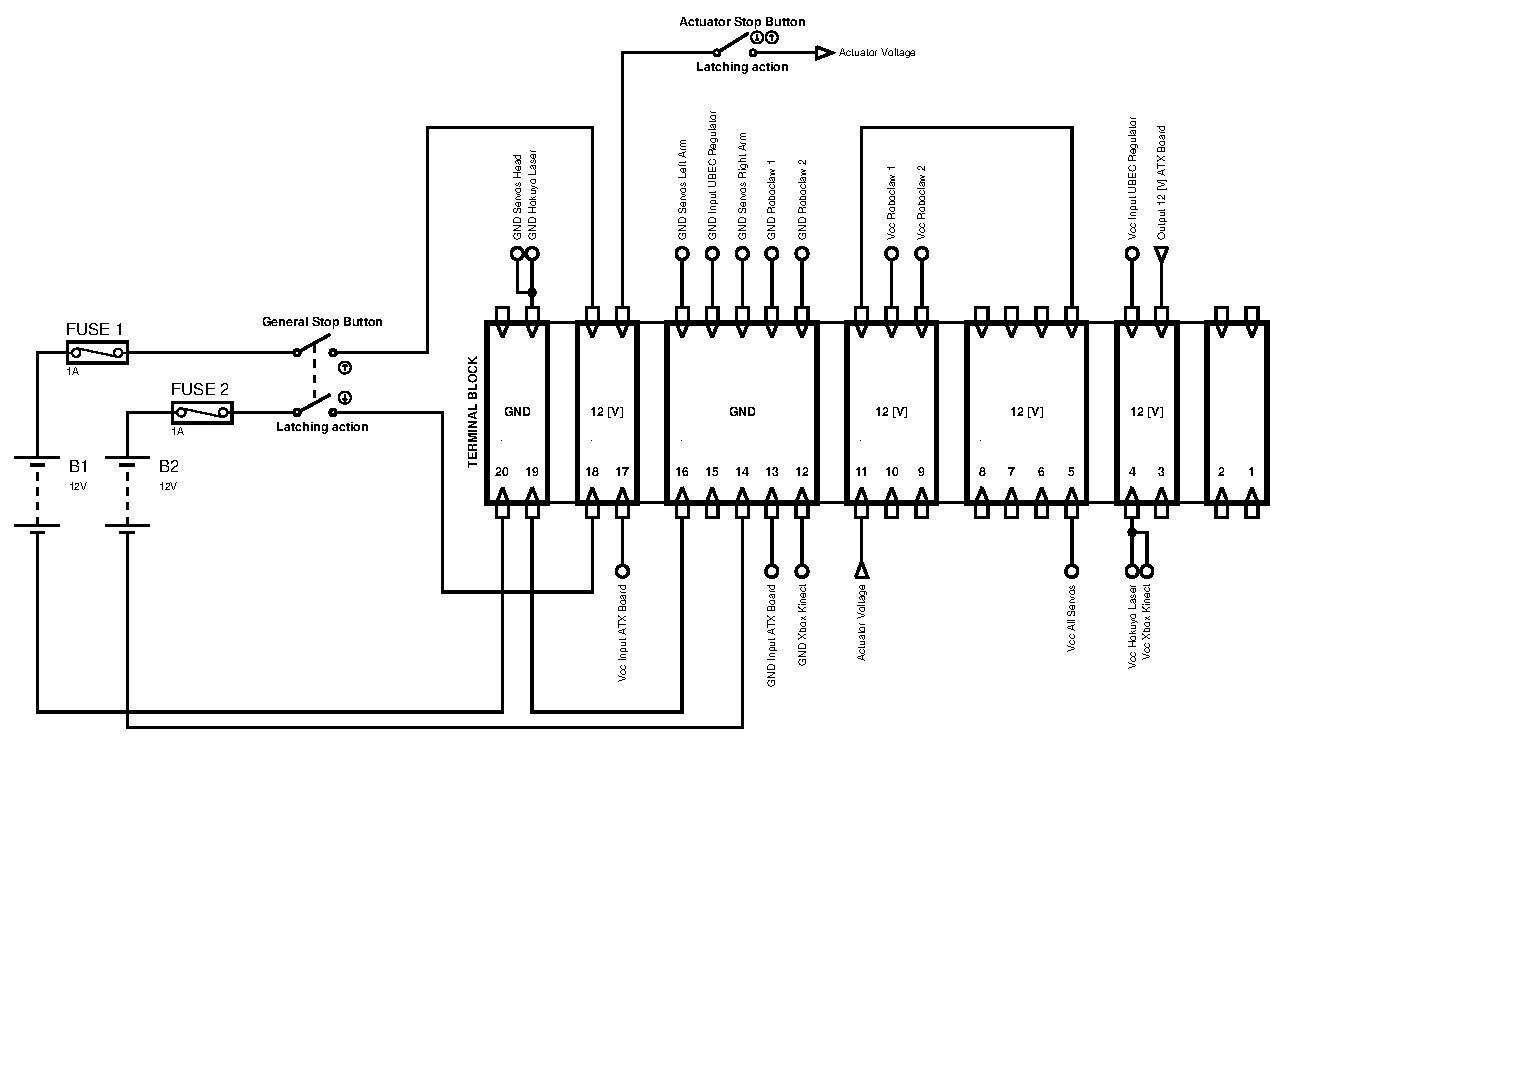
\includegraphics[width=0.8\textwidth]{Figures/Hardware/Esquematicos/JustinaWiringDiagram.jpg}
\captionof{figure}{Diagrama general}
\label{fig:Hardware:Partes:Diagrama:Esquematico:General}
\end{center}

\subsection{Diagrama esquemático Roboclaws}

%Figura
\begin{center}
\includegraphics[width=0.55\textwidth]{Figures/Hardware/Esquematicos/Roboclaw_1.png}
\captionof{figure}{Diagrama de la roboclaw 2x15A}
\label{fig:Hardware:Partes:Diagrama:Esquematico:Roboclaw:1}
\end{center}

%Figura
\begin{center}
\includegraphics[width=0.55\textwidth]{Figures/Hardware/Esquematicos/Roboclaw_2.png}
\captionof{figure}{Diagrama de la roboclaw 2x30A}
\label{fig:Hardware:Partes:Diagrama:Esquematico:Roboclaw:2}
\end{center}

\section{Comunicación hardware-computadora}
Para la conexión de Justina con la computadora se hace uso de 3 HUB los cuales están conectados de manera tal que sólo en necesario conectar
un HUB a la laptop. El primer HUB (linksys) es utilizado para conectar los actuadores de los dos brazos y la cabeza mecatronica,
el segundo HUB (el primer Startech) se utiliza para conectar las dos roboclaw, la 2x30A y la 2x15A, por ultimo tenemos el HUB (el segundo 
Startech) que es donde llegan los dos HUB anteriores así como el hokuyo y un control de xbox (que es utilizado para mover a Justina), para
ser enviado a la laptop.
\begin{center}
\includegraphics[width=0.7\textwidth]{Figures/Hardware/Diagramas/HUB.png}
\captionof{figure}{Diagrama de conexiones de los HUBs}
\label{fig:Hardware:Diagramas:Justina:HUBs}
\end{center}


\section{Interruptores de encendido y apagado}

En la base Justina cuenta con dos botones, el negro que está etiquetado como ``ON'' sirve para encender a Justina y el botón
rojo está etiquetado como ``OFF'' el cual sirve para apagar a Justina.\\

\begin{center}
\includegraphics[width=0.6\textwidth]{Figures/Hardware/Diagramas/Encendido.png}
\captionof{figure}{Encendido y apagado de Justina}
\label{fig:Hardware:Diagramas:Justina:Encendido}
\end{center}

También cuenta con dos fusibles para protección del sistema para cuando exista un mal funcionamiento en la alimentación de 
Justina. Además tiene un display el cual muestra el voltaje actual de las baterías que alimentan a Justina, esto nos sirve
para ver que el voltaje con el que cuentan las baterías no este por debajo del voltaje de operación recomendado y no cause
un mal funcionamiento en éstas.

\subsection{Boton de paro de emergencia}
El botón de paro de emergencia se encuentra a un lado del torso. La función de este botón es 
detener todos los actuadores de Justina ante una emergencia como un mal funcionamiento.
\begin{center}
\includegraphics[width=0.3\textwidth]{Figures/Hardware/Partes/RBES.jpg}
\captionof{figure}{Encendido y apagado de Justina}
\label{fig:Hardware:Partes:Paro:Boton}
\end{center}

\section{Uso y seguridad de la batería}

Es importante saber los limites y voltajes de operación recomendados por el fabricante para el correcto uso de las baterias. 
A continuación ponemos información pertinente para un correcto uso de las baterias.
%Información sobre la batería LiPo
\subsection{Instrucciones de uso y seguridad para baterías LiPo (POLÍMERO DE LITIO)}
Normas a seguir para evitar cualquier peligro o mal funcionamiento:

\begin{itemize}

    \item Emplee sólo cargadores específicos para baterías de Polímero de Litio (LiPo). En caso contrario puede provocar un 
    incendio que derive en daños personales y/o materiales.
    \item Nunca cargue las baterías LiPo sin estar presente. Siempre debe vigilar el proceso para poder reaccionar ante cualquier
    problema que se pudiese plantear.
    \item Si en cualquier momento observa que una batería Lipo se hincha o derrama líquido, desconéctela y obsérvela durante 15
    minutos en un lugar seguro y alejado de cualquier material combustible.
    \item Tenga mucho cuidado de que NUNCA se toquen los dos terminales de la batería, este cortocircuito podría hacer que la 
    batería se incendiase.
    \item Una batería que haya sufrido un golpe, cortocircuito u otro problema puede llegar a incendiarse incluso 10-15 minutos 
    después de haberse producido este hecho. Lleve rápidamente la batería a un lugar seguro y obsérvela durante 15 minutos.
    \item NUNCA almacene sus baterías en un vehículo ni en cualquier lugar donde se puedan alcanzar temperaturas altas. Las 
    temperaturas extremas pueden causar el incendio de la batería.
    \item Tenga mucho cuidado de NO PERFORAR ningún pack de baterías LiPo, puede provocar un incendio.
    \end{itemize}
    
\subsection{Proceso de carga:}
\begin{itemize}
 \item  Nunca cargue las baterías sin vigilarlas y utilice solo cargadores especiales para las baterías de lipo, así como tener
    en cuenta el número de elementos que contiene su batería.
 \item Cargue las baterías en un área segura y aislada de cualquier material inflamable.
 \item Deje enfriar la batería a la temperatura ambiente antes de comenzar la carga.
 \item Valores nominales de una batería de lipo cargada.\\
 \\
    Lipos 2S (2 elementos): entre 8,32 y 8,44V\\
    Lipos 3S (3 elementos): entre 12,48 y 12,66V\\
    Lipos 4S (4 elementos): entre 16,64 y 16,88V\\
\end{itemize}   

Nunca descargue una batería por debajo de 3V por elemento, puede dañar la batería. Para ello debe tener cuidado de no 
agotarla más de lo debido empleando dispositivos de corte por bajo voltaje o variadores especialmente diseñados para 
baterías LiPo.\\
\\
Fin de vida de las baterías LiPo:\\
\\
Cuando la capacidad de la batería haya disminuido un 30\%, deberá desecharla. Para ello descárguela a 3V por elemento, 
aísle sus terminales, envuélvala en plástico y deposítelas en los contenedores especiales para el desecho responsable de 
pilas.\\

\section{Precauciones y conexión de la Roboclaw}

\subsection{Precauciones}
Estas son precauciones sumamente importantes que se deberán seguir para evitar daños a la Roboclaw y los sistemas conectados.\\
\\
1. Desconectar la terminal negativa de la alimentación no es la mejor forma para apagar el motor. Si conectas cualquier entrada o salida
a la Roboclaw obtienes un ciclo de tierra a los pines de entrada/salida como resultado. Puede causar daños a la Roboclaw y cualquier
dispositivo conectado. Para apagar el controlador del motor debe removerse primero la conexión positiva de la alimentación después de
que los motores dejen de moverse.\\
\\
2. El motor de DC puede trabajar como un generador cuando este gira. Siempre detenga el motor
antes de apagar la Roboclaw.\\
\\
3. Apagar en caso de emergencia, un interruptor y/o contacto de un tamaño adecuado debe ser utilizado. Se debe usar un diodo correcto para
hacer un puente entre el apagador y el contacto.\\
\\
4. Dependiendo del modelo de RoboClaw hay un requisito mínimo de potencia de al menos 6V. Bajo cargas pesadas, si la batería lógica y
la batería principal se combinan, pueden suceder caídas de tensión. Esto puede causar un comportamiento errático de la RoboClaw.\\
Vista general de los conectores\\
\\
En el control principal de entrada/salida, están puestos para una fácil conectividad para controlar dispositivos como controladores RC.
Los cabezales están también arreglados para proveer un fácil acceso a tierra  y alimentación para suministrar poder a controladores externos.

\begin{center}
\includegraphics[width=0.9\textwidth]{Figures/Hardware/Partes/Pines.png}
\captionof{figure}{Configuración de pines}
\label{fig:Hardware:Partes:Pines}
\end{center}

Bateria lógica (LB IN)\\
La parte lógica de la RoboClaw puede ser alimentada por una batería secundaria conectada a LB IN. La terminal positiva
(+) está localizada al borde de la tarjeta y la tierra (-) es el pin más cercano al disipador. Remueva el jumper LB-MB
para que la batería secundaría pueda ser usada.\\
\\
Encoder power (+ -)\\
Los pines marcados como (+) y (–) son los pines de alimentación  de los encoders. El positivo (+) está localizado al
borde de la tarjeta y la fuente +5VDC. El pin de tierra (-) está cercano al disipador. En todos los modelos ST la
alimentación debe venir del único borne de 5v  y a GND\\
\\
Entradas de los encoder (EN1 / EN2 – 1B / 1A / 2B / 2A)\\ 
EN1 y EN2 son las entradas de los enconders en versión pin del RoboClaw. 1B, 1A, 2B y 2A son las entradas de los encoders
a los bornes de la RoboClaw. El canal A de ambos EN1 y EN2 están localizados en los pines del borde de la tarjeta.
Los pines del canal B están localizados cercanos al disipador en los pines. Los canales A y B están debidamente etiquetados
en los bornes.\\
\\
Cuando conectes los encoders asegúrese que el canal para la dirección de giro esté conectado en A. si un encoder es
llevado hacia atrás a el otro, tendrás un contador interno que contara hacía adelante y hacia atrás. \\
\\
Control de entradas (S1 / S2 / S3 / S4 / S5)\\
S1, S2, S3, S4 y S5 están configuradas para pines de servo estándar de estilo (tipo) entrada/salida (excepto en modelos ST)
, +5V y GND. S1 y S2 son las entradas  de los modos de control serial, analógico y RC. S3, S4 y S5 pueden ser usadas como
entrada de corte de emergencia o como salidas de control de voltaje.\\
\\
Bornes de la batería principal\\
La alimentación de entrada principal puede ser desde 6VDC a 34VDC en la RoboClaw estándar y de 10.5VDC a 60VDC en la Roboclaw
de alto voltaje. Las conexiones son hechas en los bornes principales (+) y (-). El símbolo de mas (+) marca la terminal
positiva y el negativo (–) marca la terminal negativa. El cableado de la batería principal debe ser lo más corto posible \\
\\
Desconectar\\
La batería principal debe ser desconectada en caso de situaciones donde se salga de control y la energía necesite ser
cortada. El interruptor debe estar estimado para manejar la máxima corriente y voltaje de la batería. Esto puede variar
dependiendo del tipo de motores y/o la fuente de alimentación que se este utilizando.\\
\\
Bornes del motor\\
Los bornes del motor están hechos con M1A/M1B para el canal 1 y M2A/M2B para el canal 2. Para que ambos motores giren en
la misma dirección, el cableado de uno de los motores debe ser contrario hacia el otro en un robot diferencial típico. El
cableado de los motores y la batería deben ser lo más cortos posibles. Los cables largos pueden incrementar la inductancia
y por lo tanto incrementan potencialmente los picos de voltaje perjudiciales.\\
\\
Leds de estado y error\\
La Roboclaw tiene tres leds. Dos leds de estado, STAT1 y STAT2, y un led de error ERR. Cuando la Roboclaw es alimentada por
primera vez, hasta los 3 leds deben parpadear brevemente para indicar que todos los led están funcionando. Los leds se
comportaran diferentemente dependiendo en qué modo está configurada la Roboclaw.\\
\\
Cableado básico\\
El diagrama de cableado de abajo ilustra la batería básica y conexiones de motor para la Roboclaw. M1A y M1B es el canal
de motor 1, junto a M2A y M2B como canal del motor 2.\\

%Figura
\begin{center}
\includegraphics[width=0.8\textwidth]{Figures/Hardware/Partes/Motores.png}
\captionof{figure}{Conexión básica de motores}
\label{fig:Hardware:Partes:Motores}
\end{center}

\textbf{Nunca desconecte la terminal negativa de la batería antes de desconectar la positiva.}\\
\\

\subsection{Modo de conexión de la roboclaw}




 
\end{document}
%Modos de la Roboclaw\\ 
%Hay 4 modos principal totalmente variables con 14 modos en total. Cada modo habilita la Roboclaw para ser controlada en una
%forma específica. La lista a continuación explica cada modo y su aplicación.\\
%El USB puede ser conectado en cualquier modo. Cuando la Roboclaw no está en modo USB serie, comandos del pack serial  pueden
%ser usados para leer información de estados y configuraciones de ajuste, sin embargo los comandos de movimiento de los motores
%no funcionaran. Cuando en el modo pack serial otro dispositivo como un arduino es conectado en los pines S1 y S2, y se
%envían comandos a la Roboclaw, ambos comandos son ejecutados.\\

%1. Modo RC 1 y 2- Con el modo RC la Roboclaw puede ser controlada por cualquier sistema de radio RC. El modo de entrada RC
%también permite microcontroladores de baja potencia como sello básico de control a la Roboclaw. La Roboclaw espera pulsos
%de entrada al servo para controlar la dirección y velocidad. Muy similar como regular un servo.\\

%2. Modo análogo 3 y 4 – El modo Análogo usa una señal analógica de 0v a 2v para controlar la velocidad y dirección de cada
%motor. La Roboclaw puede ser controlada usando un potenciómetro o un PWM filtrado por un microcontrolador. El modo análogo
%es ideal para interfaces de la Roboclaw con sistemas de posicionamiento con joysticks u otro hardware de interfaz sin
%microcontrolador. El modo análogo puede usar encoders si tiene la configuración indicada.\\

%3. Modo serial estándar 5 y 6 – En el modo serial estándar la Roboclaw espera datos nivel TTL serial del RS-232 para
%controlar dirección y velocidad de cada motor. El serial estándar es típicamente usado para controlar la Roboclaw desde
%un microcontrolador o PC. Si se usa una PC, un MAX232 o un circuito convertidor de nivel equivalente debe ser usado desde
%la Roboclaw la cual sólo trabaja con entradas de nivel TTL. El serial estándar incluye un modo de selección esclavo el 
%cual permite controlar múltiples Roboclaw por una señal desde el puerto RS-232 (PC o microcontrolador). El serial estándar
%es un formato de un solo camino, la Roboclaw sólo recibe datos. Los encoders no tienen soporte  con el modo serial estándar.\\

%4. Modo serial por paquetes del 7 al 14 – En el modo serial de paquetes la Roboclaw espera datos de nivel TTL serial del 
%RS-323 para controlar dirección y velocidad de cada motor. Los paquetes serial son típicamente usados para controlar la 
%Roboclaw desde un microcontrolador o PC. Si se usa una PC, un MAX232 o un circuito convertidor equivalente debe ser usado 
%desde la Roboclaw ya que trabaja sólo con entradas de nivel TTL. En el modo seria por paquetes cada Roboclaw tiene asignada
%una dirección única. Existen 8 direcciones disponibles. Esto significa que hasta 8 Roboclaws pueden ser usadas en el mismo 
%puerto serial. Los encoders tienen soporte en éste modo.\\

%5. Control USB – El USB puede ser conectado en cualquier modo. Cuando la Roboclaw no está en modo serial por paquetes los
%comandos serial pueden ser utilizados para leer información de estados y/o configurar ajustes, sin embargo los comandos de 
%movimiento del motor no funcionaran. Cuando en el modo serial por paquetes hay otro dispositivo, como por ejemplo arduino, 
%es conectado a los pines S1 y S2, y envía ambos comandos a la Roboclaw y los comandos serial por paquetes USB son ejecutados.\\
%Aquí terminan los consejos de la roboclaw
